\documentclass[border=4pt]{standalone}

\usepackage{amsmath}
\usepackage{tikz}
\usepackage{mathdots}
\usepackage{yhmath}
\usepackage{cancel}
\usepackage{color}
\usepackage{siunitx}
\usepackage{array}
\usepackage{multirow}
\usepackage{amssymb}
\usepackage{gensymb}
\usepackage{tabularx}
\usepackage{booktabs}
\usetikzlibrary{fadings}
\usetikzlibrary{patterns}


\begin{document}
 \tikzset{every picture/.style={line width=0.75pt}} %set default line width to 0.75pt

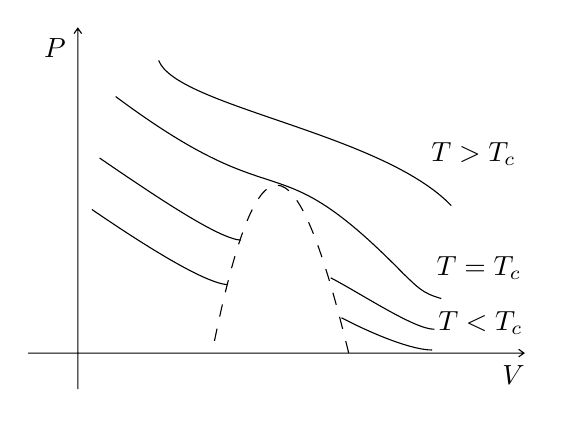
\begin{tikzpicture}[x=0.75pt,y=0.75pt,yscale=-0.37,xscale=0.37]
%uncomment if require: \path (0,476); %set diagram left start at 0, and has height of 476

%Shape: Axis 2D [id:dp5951100625553807]
\draw  (12.61,425) -- (658.18,425)(77.17,2) -- (77.17,472) (651.18,420) -- (658.18,425) -- (651.18,430) (72.17,9) -- (77.17,2) -- (82.17,9)  ;
%Curve Lines [id:da2126694468363458]
\draw    (563.5,233) .. controls (472.5,138) and (205.5,104) .. (182.5,44) ;


%Curve Lines [id:da8602998139648838]
\draw  [dash pattern={on 4.5pt off 4.5pt}]  (429.9,424.97) .. controls (359.9,136.97) and (310.9,129.97) .. (251.9,424.97) ;


%Shape: Boxed Bezier Curve [id:dp6932412254916785]
\draw    (501.5,322) .. controls (326.5,143) and (349.5,257) .. (126.5,91) ;


%Curve Lines [id:da8502267220518913]
\draw    (289.5,278) .. controls (260.5,276) and (181.5,223) .. (105.5,171) ;


%Curve Lines [id:da8746517244181468]
\draw    (272.5,336) .. controls (243.5,334) and (171.5,290) .. (95.5,238) ;


%Curve Lines [id:da4382617853232931]
\draw    (538.5,421) .. controls (512.5,421) and (462.5,401) .. (420.5,379) ;


%Curve Lines [id:da368608553657754]
\draw    (541.5,394) .. controls (515.5,394) and (448.5,349) .. (406.5,327) ;


%Curve Lines [id:da19861479220559797]
\draw    (550.5,354) .. controls (525.5,347) and (519.5,339) .. (501.5,322) ;



% Text Node
\draw (47.5,27.32) node [scale=1]  {$P$};
% Text Node
\draw (644.64,453.88) node [scale=1]  {$V$};
% Text Node
\draw (601.49,385.88) node [scale=1]  {$T< T_{c}$};
% Text Node
\draw (599.49,313.88) node [scale=1]  {$T=T_{c}$};
% Text Node
\draw (592.49,165.88) node [scale=1]  {$T >T_{c}$};


\end{tikzpicture}

\end{document}
